\documentclass[12pt]{article}
\usepackage[table]{xcolor}
\usepackage[margin=1in]{geometry} 
\usepackage{amsmath,amsthm,amssymb}
\usepackage[english]{babel}
\usepackage{tcolorbox}
\usepackage{enumitem}
\usepackage{hyperref}
\usepackage{listings}
\usepackage{blkarray}
\usepackage{float}
\usepackage{bm}
\usepackage{subfigure}
\usepackage{tikz}
\usetikzlibrary{trees}
\usepackage{booktabs}
\usepackage{siunitx}
\usepackage{url}

\setcounter{secnumdepth}{5}
\setcounter{tocdepth}{5}

\newtheorem{theorem}{Theorem}[section]
\newtheorem{corollary}{Corollary}[theorem]
\newtheorem{lemma}[theorem]{Lemma}
\newtheorem{proposition}[theorem]{proposition}
\newtheorem{exmp}{Example}[section]\newtheorem{definition}{Definition}[section]
\newtheorem{remark}{Remark}
\newtheorem{ex}{Exercise}
\theoremstyle{definition}
\theoremstyle{remark}
\bibliographystyle{elsarticle-num}

\DeclareMathOperator{\sinc}{sinc}
\newcommand{\RNum}[1]{\uppercase\expandafter{\romannumeral #1\relax}}
\newcommand{\N}{\mathbb{N}}
\newcommand{\Z}{\mathbb{Z}}
\newcommand{\R}{\mathbb{R}}
\newcommand{\E}{\mathbb{E}}
\newcommand{\matindex}[1]{\mbox{\scriptsize#1}}
\newcommand{\V}{\mathbb{V}}
\newcommand{\Q}{\mathbb{Q}}
\newcommand{\K}{\mathbb{K}}
\newcommand{\C}{\mathbb{C}}
\newcommand{\prob}{\mathbb{P}}

\lstset{numbers=left, numberstyle=\tiny, stepnumber=1, numbersep=5pt}

\setcounter{secnumdepth}{0}

\begin{document}
\sloppy
\title{SOC of Renewable Energy: ReadMe}
\author{Renzo Miguel Caballero Rosas} 
\maketitle

\tableofcontents

\section{Functions}

\tikzstyle{every node}=[draw=black,thick,anchor=west]
\tikzstyle{selected}=[draw=red,fill=red!30]
\tikzstyle{optional}=[dashed,fill=gray!50]
%child { node [selected] {tex}
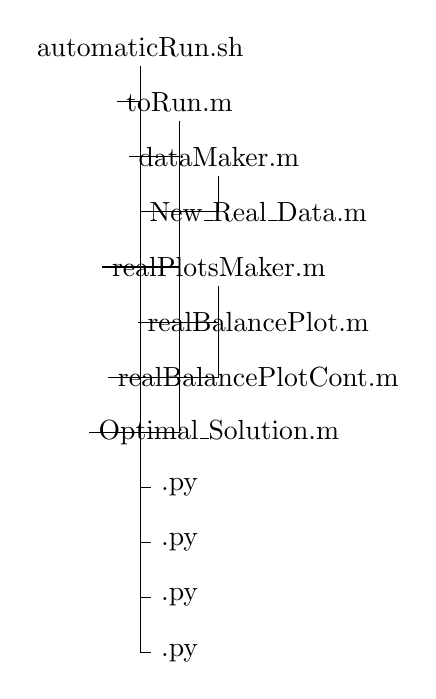
\begin{tikzpicture}[%
  grow via three points={one child at (0.5,-0.7) and
  two children at (0.5,-0.7) and (0.5,-1.4)},
  edge from parent path={(\tikzparentnode.south) |- (\tikzchildnode.west)}]
  \node {automaticRun.sh}
  child { node {toRun.m}
      child { node {dataMaker.m}
      		child { node  {New\_Real\_Data.m}}}
      child [missing] {}	
      child { node  {realPlotsMaker.m}
      		child { node {realBalancePlot.m}}
      		child { node {realBalancePlotCont.m}}}
      		child [missing] {}	
      		child [missing] {}	
      child { node {Optimal\_Solution.m}}
    }
    child [missing] {}	
    child [missing] {}				
    child [missing] {}
    child [missing] {}	
    child [missing] {}					
    child [missing] {}	
    child { node {.py}}		
    child { node {.py}}
    child { node {.py}}			
    child { node {.py}};
\end{tikzpicture}

\section{Used Data}

All the data used is from official sources. Here we will show which data we use, from where we obtain it and how.\\
We have two kinds of data, the one used to construct the mathematical models (call it \textbf{model data}) and the one needed to compute the daily simulations (call it \textbf{daily data}). The \textbf{model data} is a \textit{single use} data, once we have constructed our models we do not need it anymore (except to do maybe some debugging). On the other hand, each day we need a different set of \textbf{daily data}, for this reason, we download it from the internet every day and just after we run the simulation.

\subsection{Daily Data}

The primary input to the simulator is a .mat file called Day\_yyyymmdd.mat, where yyyymmdd is the date of the corresponding day (i.e., the first of Febrary 2019 would have $yyyymmdd=20190201$). The function that creates this file is \textbf{New\_Real\_Data.m}, where we can introduce the date that we want (in format $[yyyy,MM,dd,hh,mm,ss]$) and it uses all the data to create the file .mat.\\
To create many files at the same time we use the script \textbf{dataMaker.m}, where we introduce the range that we want to create.\\
When we load this file into MATLAB, we obtain a $1\times9$ cell called \textbf{Matrix} which contains all the daily data needed. Each element in this cell corresponds to specific data, which is fundamental to run the simulation. Now we will see the information corresponding to each element:

\subsubsection{Matrix\{1\}:}

\begin{enumerate}

\item[$\bullet$] Structure: Array with dimensions $145\times89$ with all the historical power balance from 00:00 to 24:00 and a frequency of 6 points per hour ($24\times6+1=145$).\\
In the first 12 columns we can find:\\
{\color{blue} (1) Salto Grande power, (2) Bonete power, (3) Baygorria power, (4) Palmar power, (5) Wind power, (6) Solar power, (7) Fossil fuel power, (8) Biomass power (9) Import Argentina, (10) Import Brazil (Rivera), (11) Import Brazil (Melo), (12) Demand}.\\
The next 42 ({\color{blue} from 13 to 54}) columns correspond to wind power per farm.\\
The next 13 ({\color{blue} from 55 to 67}) columns correspond to solar power per farm.\\
The next 7 ({\color{blue} from 68 to 74}) columns correspond to fossil fuel power per station. We can find:\\
{\color{blue} (68) Zenda, (69) PTA6, (70) Motores, (71) CTR, (72) PTB, (73) PTA7\&8, (74) ???}.\\
The next 9 ({\color{blue} from 75 to 83}) columns correspond to biomass power per station.\\
The last 6 columns correspond to the imports and exports of power. We can find:\\
{\color{blue} (84) Export Brazil (Melo), (85) Export Brazil (Rivera), (86) Export Argentina, (87) Import Brazil (Melo), (88) Import Brazil (Rivera), (89) Import Argentina}.\\

\item[$\bullet$] Webpage: In {\color{blue} \url{https://pronos.adme.com.uy/gpf.php}}, we can download all this data using the button \textit{Archivo Scada Detalle}. Also, it is possible to choose the range that we want to download.

\item[$\bullet$] Raw data location: After we download the data, we save it in \textbf{.../Dropbox/Python/Represas\_Data\_2/ADME\_Historicos/yyyymmdd.ods}. We respect the original format and save in .ods. However, we have to change the sheet names because they have Spanish accents, then we save the modified ones as \textbf{.../Dropbox/Python/Represas\_Data\_2/ADME\_Historicos\_Corrected/yyyymmdd.ods}.

\item[$\bullet$] Web scraper: The script used to download the data is \textbf{.../Dropbox/Python/Represas\_Data\_2/ADME\_Historicos\_de\_Produccion\_ODS.ipynb}. The automatic version has the same name and location but extension \textbf{.py}, it downloads all from 03/11/2016 to two day before the actual date.\\
After we run the modification. The script is \textbf{.../Dropbox/Python/Represas\_Data\_2/changeOdsSheetName.ipynb} (the automatic version is the same but with \textbf{.py}).

\end{enumerate}

\subsubsection{Matrix\{2\}:}

\begin{enumerate}

\item[$\bullet$] Structure: Array with dimensions $1\times10$ with the needed daily data from the fossil fuel power plants.\\
The data is [\textbf{{\color{blue} CTR\_Cost, CTR\_MaxPower, Motores\_Cost, Motores\_MaxPower, PTA6\_Cost, PTA6\_MaxPower, PTB\_Cost, PTB\_MaxPower, PTA7\&8\_Cost, PTA7\&8\_MaxPower}]}.
\item[$\bullet$] Webpage: In {\color{blue} \url{https://adme.com.uy/mmee/cvr.php}}, we can download the cost of the resources. The maximum power (until now) only can be found in SimSEE.

\item[$\bullet$] Raw data location: The costs and maximum power can be find in \textbf{.../Dropbox/SOC\_of\_Renewable\_Energy/Data\_Valores/Termicas\_ADME.xlsx} and \textbf{.../Dropbox/SOC\_of\_Renewable\_Energy/Data\_Valores/Termicas\_SimSEE.xlsx}, respectively.

\item[$\bullet$] Web scraper: The script used to download \textbf{the costs} is \textbf{.../Dropbox/SOC\_of\_Renewable\_Energy/Data\_Valores/dataADME.ipynb}. The automatic version has the same name and location but extension \textbf{.py}, it downloads all from 01/01/2018 to two day before the actual date. {\color{red} The problem with \textbf{the max power} is that it is inside SimSEE}.\\
In this case, the automatic version needs the existence of a base \textbf{.xlsx}. It does not create the \textbf{.xlsx} file, only reads and writes it.

\end{enumerate}

\subsubsection{Matrix\{3\}:}

\begin{enumerate}

\item[$\bullet$] Structure: Array with dimensions $1\times4$ with the water value.\\
The data is [\textbf{{\color{blue} WaterValue\_SG, WaterValue\_Palmar, WaterValue\_Bonete, WaterValue\_Baygorria}]}.

\item[$\bullet$] Webpage: In {\color{blue} \url{https://adme.com.uy/mmee/cvr.php}}, we can download the cost of the resources.

\item[$\bullet$] Raw data location: The water value can be find in \textbf{.../Dropbox/SOC\_of\_Renewable\_Energy/Data\_Valores/Valores\_de\_Agua\_ADME.xlsx}.

\item[$\bullet$] Web scraper: \item[$\bullet$] Web scraper: The script used to download \textbf{the costs} is \textbf{.../Dropbox/SOC\_of\_Renewable\_Energy/Data\_Valores/dataADME.ipynb}. The automatic version has the same name and location but extension \textbf{.py}, it downloads all from 01/01/2018 to two day before the actual date.\\
In this case, the automatic version needs the existence of a base \textbf{.xlsx}. It does not create the \textbf{.xlsx} file, only reads and writes it.

\end{enumerate}

\subsubsection{Matrix\{4\}:}

\begin{enumerate}

\item[$\bullet$] Structure: Array with dimensions $1\times3$ with the initial volume of Bonete (in $\SI{}{hm^3}$) and the daily average natural inflow (in $\SI{}{hm^3}$), and the daily spilled water (in $\SI{}{hm^3}$).\\
The data is [\textbf{{\color{blue} Bonete\_InitialVolume, Bonete\_DailyInflow, Bonete\_DailySpilled}]}.

\item[$\bullet$] Webpage: In {\color{blue} \url{https://apps.ute.com.uy/SgePublico/ConsBalanceHid.aspx}}, we can download the next data: {\color{orange} Volumen Inicial Embalsado, Volumen Final Embalsado, Gasto de Agua,  Volumen Turbinado, Volumen Vertido, Volumen Filtrado, Volumen Evaporado, Aporte Te\'orico}.

\item[$\bullet$] Raw data location: The initial volume and natural inflow of Bonete can be found in \textbf{.../Dropbox/Python/Represas\_Data\_2/Bonete\_Data.xls}.

\item[$\bullet$] Web scraper: The script used to download the data is \textbf{.../Dropbox/Python/Represas\_Data\_2/Bonete\_Data\_2.ipynb}. The automatic version is in the same folder, but with name \textbf{Bonete\_Data\_Automatic.py}. To download automatically it is necessary that the file \textbf{.xls} exists and it must have data until 2019 at least, the script downloads from 2019 to two days before the actual date.

\end{enumerate}

\subsubsection{Matrix\{5\}:}

\begin{enumerate}

\item[$\bullet$] Structure: Array with dimensions $1\times3$ with the initial volume of Baygorria (in $\SI{}{hm^3}$) and the daily average natural inflow (in $\SI{}{hm^3}$), and the daily spilled water (in $\SI{}{hm^3}$).\\
The data is [\textbf{{\color{blue} Baygorria\_InitialVolume, Baygorria\_DailyInflow, Baygorria\_DailySpilled}]}.

\item[$\bullet$] Webpage: In {\color{blue} \url{https://apps.ute.com.uy/SgePublico/ConsBalanceHid.aspx}}, we can download the next data: {\color{orange} Volumen Inicial Embalsado, Volumen Final Embalsado, Gasto de Agua,  Volumen Turbinado, Volumen Vertido, Volumen Filtrado, Volumen Evaporado, Aporte Te\'orico}.

\item[$\bullet$] Raw data location: The initial volume and natural inflow of Baygorria can be found in \textbf{.../Dropbox/Python/Represas\_Data\_2/Baygorria\_Data.xls}.

\item[$\bullet$] Web scraper: The script used to download the data is \textbf{.../Dropbox/Python/Represas\_Data\_2/Baygorria\_Data\_2.ipynb}. The automatic version is in the same folder, but with name \textbf{Baygorria\_Data\_Automatic.py}. To download automatically it is necessary that the file \textbf{.xls} exists and it must have data until 2019 at least, the script downloads from 2019 to two days before the actual date.

\end{enumerate}

\subsubsection{Matrix\{6\}:}

\begin{enumerate}

\item[$\bullet$] Structure: Array with dimensions $1\times3$ with the initial volume of Palmar (in $\SI{}{hm^3}$), the daily average natural inflow (in $\SI{}{hm^3}$), and the daily spilled water (in $\SI{}{hm^3}$).\\
The data is [\textbf{{\color{blue} Palmar\_InitialVolume, Palmar\_DailyInflow, Palmar\_DailySpilled}]}.

\item[$\bullet$] Webpage: In {\color{blue} \url{https://apps.ute.com.uy/SgePublico/ConsBalanceHid.aspx}}, we can download the next data: {\color{orange} Volumen Inicial Embalsado, Volumen Final Embalsado, Gasto de Agua,  Volumen Turbinado, Volumen Vertido, Volumen Filtrado, Volumen Evaporado, Aporte Te\'orico}.

\item[$\bullet$] Raw data location: The initial volume and natural inflow of Palmar can be found in \textbf{.../Dropbox/Python/Represas\_Data\_2/Palmar\_Data.xls}.

\item[$\bullet$] Web scraper: The script used to download the data is \textbf{.../Dropbox/Python/Represas\_Data\_2/Palmar\_Data\_2.ipynb}. The automatic version is in the same folder, but with name \textbf{Palmar\_Data\_Automatic.py}. To download automatically it is necessary that the file \textbf{.xls} exists and it must have data until 2019 at least, the script downloads from 2019 to two days before the actual date.

\end{enumerate}

\subsubsection{Matrix\{7\}:}

\begin{enumerate}

\item[$\bullet$] Structure: Array with dimensions $1\times2$ with the average daily inflow of Salto Grande (in $\SI{}{m^3/s}$) and its initial level (in $\SI{}{m}$).\\
The data is [\textbf{{\color{blue} SG\_AverageDailyInflow, SF\_InitialLevel}]}.

\item[$\bullet$] Webpage: The webpages from we download the average natural inflow and initial level are {\color{blue} \url{https://www.saltogrande.org/datos_diarios.php}} and {\color{blue} \url{https://apps.ute.com.uy/SgePublico/ConsNivelesPresasHoraria.aspx}}, respectively.

\item[$\bullet$] Raw data location: The average natural inflow and initial level of Salto Grande can be found in \textbf{.../Dropbox/Python/Represas\_Data\_2/SG\_Data/yymmdd.csv} and \textbf{.../Dropbox/Python/Represas\_Data\_2/Salto\_Grande\_Data\_Horaria.csv}, respectively.

\item[$\bullet$] Web scraper: The script used to download the average natural inflow and initial level are \textbf{.../Dropbox/Python/Represas\_Data\_2/SaltoGrande\_Data.ipynb} and \textbf{.../Dropbox/Python/Represas\_Data\_2/Salto\_Grande\_Data\_Horaria.ipynb}, respectively. \textbf{SaltoGrande\_Data.py} and \textbf{Salto\_Grande\_Data\_Horaria\_Automatic.py} are the respective automatic versions. The second one needs the existence of the file \textbf{.csv}.

\end{enumerate}

\subsubsection{Matrix\{8\}:}

\begin{enumerate}

\item[$\bullet$] Structure: Array with dimensions $25\times8$ with hourly data (from 00:00 to 24:00). This array contains the level of the dams upstream and downstream. Also, it has the gap existing between the level downstream and upstream of concatenated dams.\\
The data is [\textbf{{\color{blue} h0\_3, h0\_4, X, X, X, X, X, X, $\Delta$BoneteBaygorria, $\Delta$BaygorriaPalmar}]}.\\
h0\_3 and h0\_4 are the level downstream of Palmar and Salto Grande, respectively. $\Delta$BoneteBaygorria is the difference between the level downstream of Bonete, and the level upstream of Baygorria.

\item[$\bullet$] Webpage: We download the levels upstream and downstream of all dams from {\color{blue} \url{https://apps.ute.com.uy/SgePublico/ConsNivelesPresasHoraria.aspx}}.

\item[$\bullet$] Raw data location: The levels upstream and downstream can be found in the files \textbf{Bonete\_Data\_Horaria.csv}, \textbf{Baygorria\_Data\_Horaria.csv}, \textbf{Palmar\_Data\_Horaria.csv} and \textbf{Salto\_Grande\_Data\_Horaria.csv}. These files are located in \textbf{.../Dropbox/Python/Represas\_Data\_2/}.

\item[$\bullet$] Web scraper: The scripts used to download the levels are \textbf{Bonete\_Data\_Horaria.ipynb}, \textbf{Baygorria\_Data\_Horaria.ipynb}, \textbf{Palmar\_Data\_Horaria.ipynb} and \textbf{Salto\_Grande\_Data\_Horaria.ipynb}. These scripts are located in \textbf{.../Dropbox/Python/Represas\_Data\_2/}. The automatic versions are in the same directory, but with names \textbf{Bonete\_Data\_Horaria\_Automatic.py}, \textbf{Baygorria\_Data\_Horaria\_Automatic.py}, \textbf{Palmar\_Data\_Horaria\_Automatic.py} and \textbf{Salto\_Grande\_Data\_Horaria\_Automatic.py}. All of them need the existence of the \textbf{.csv} file to work properly and they download until two days before the actual date.

\end{enumerate}

\subsubsection{Matrix\{9\}:}

\begin{enumerate}

\item[$\bullet$] Structure: Array with dimensions $61\times2$ with hourly data with a frequency of 6 points per hour (from 14:00 to 24:00). The data is the average of all the flow (in $\SI{}{m^3/s}$) in the previous day for Bonete and Baygorria.\\
The data is [{\color{blue} AveragedTotalFlowBonete, AveragedTotalFlowBaygorria}].\\
This averaged flow is used as the virtual flow for Baygorria (the water from Bonete) and Palmar (the water from Baygorria).

\item[$\bullet$] Webpage: We download the used water from the webpage {\color{blue} \url{https://apps.ute.com.uy/SgePublico/ConsBalanceHid.aspx}}.

\item[$\bullet$] Raw data location: The used water of Bonete and Baygorria can be found in \textbf{.../Dropbox/Python/Represas\_Data\_2/Bonete\_Data.xls} and \textbf{.../Dropbox/Python/Represas\_Data\_2/Baygorria\_Data.xls}, respectively.

\item[$\bullet$] Web scraper: The scripts used to download data of Bonete and Baygorria are \textbf{.../Dropbox/Python/Represas\_Data\_2/Bonete\_Data\_2.ipynb} and \textbf{.../Dropbox/Python/Represas\_Data\_2/Baygorria\_Data\_2.ipynb}, respectively.  The automatic versions are in the same folder, but with names \textbf{Bonete\_Data\_Automatic.py} and \textbf{Baygorria\_Data\_Automatic.py}. To download automatically it is necessary that the files \textbf{.xls} exist and they must have data until 2019 at least, the scripts download from 2019 to two days before the actual date.

\end{enumerate}

\section{MaxFlowCoeff.mat}

This file is created using \textbf{Approximation.m} in \textbf{Dropbox/Thesis Research/Datos centrales eléctricas - UTE/Despacho de Cargas}.

\section{Real$\_$Data.m}

This script creates real data plots, and also, it creates the files with all the needed information for each day.

\section{New$\_$Real$\_$Data.m}

This script uses the data in the format that python downloads. The idea is that we downloas with python, this script created the daily matrix and after, all the simulation is done in Ibex (cluster of KAUST).

\section{Valores de Agua}

See \url{latorre.adme.com.uy/vates/15253/hoja_ValoresAguaPromedio.xlt}.

\section{What if $[\text{Valores de Agua}] = 0$?}

In this case, if the system never uses fuel (which has cost different of zero), then the opportunity cost for the water will always be zero. However, in this case, we can increase the exports and force the system to use fuel, which will change the opportunity cost for the water and then, we would use it optimally.

\section{How do we know we are optimal?}

Puedo modificar los valores de las derivadas parciales. Si hago eso, al resolver forward voy a encontrar controles admisibles que en teor\'ia no ser\'ian \'optimos. Luego coloco esos controles usando las verdaderas derivadas parciales y me fijo cuanto es el costo para comparar.

\section{Matrix with Daily Data (i.e.: Day$\_$6$\_$2019.mat)}

This is the matrix which the script \textbf{Optimal\_Solution.m} will read. This matrix is a cell where each camp has an array or cell inside. The data inside each cell is:

\begin{enumerate}

\item Array with dimensions $145\times16$. The 145 corresponds of 24 hours with frequency 6 points per hour (from 00:00 to 24:00). The 16 are: \textbf{[Fecha, Salto Grande, Bonete, Baygorria, Palmar, E\'olica, Solar, T\'ermica, Biomasa,	Imp.Arg, Imp.Br.Riv, Imp.Br.Mel, Demanda, Exp\_Intercon\_BR\_MELO, Exp\_Intercon\_BR\_RIVERA, Exp\_Intercon\_ARG]}.\\
{\color{red} Modified version}: Array with dimensions $145\times89$. \textbf{[{\color{blue} (1) Salto Grande, (2) Bonete, (3) Baygorria, (4) Palmar, (5) E\'olica, (6) Solar, (7) T\'ermica, (8) Biomasa (9) Imp.Arg, (10) Imp.Br.Riv, (11) Imp.Br.Mel, (12) Demanda},\\
X,\\
X,\\
X,\\
X,\\
{\color{blue} (84) Exp\_Intercon\_BR\_MELO, (85) Exp\_Intercon\_BR\_RIVERA,\\
 (86) Exp\_Intercon\_ARG, (87) Imp\_Intercon\_BR\_MELO,\\
  (88) Imp\_Intercon\_BR\_RIVERA, (89) Imp\_Intercon\_ARG}]}.

\item Array with dimensions $1\times8$. The data is \textbf{[CTR\_Cost, CTR\_MaxPower, Motores\_Cost, Motores\_MaxPower, PTA\_Cost, PTA\_MaxPower, PTB\_Cost, PTB\_MaxPower]}.

\item Array with dimensions $1\times3$. The data is \textbf{[WaterValue\_SG, WaterValue\_Palmar, WaterValue\_Bonete]}.

\item Array with dimensions $1\times2$. The data is the initial volume (in $\SI{}{hm^3}$) and the average natural flow (in $\SI{}{hm^3}$) for \textbf{Bonete}.

\item Array with dimensions $1\times2$. The data is the initial volume (in $\SI{}{hm^3}$) and the average natural flow (in $\SI{}{hm^3}$) for \textbf{Baygorria}.\\
{\color{red} Notice that}: To compute the natural inflow of Baygorria, I use the theoretical inflow (which is all the water that theoretically entered during the day) and I substrate the water used in Bonete (I subtract 6/24 from the day before, and 18/24 from the actual day).

\item Array with dimensions $1\times2$. The data is the initial volume (in $\SI{}{hm^3}$) and the average natural flow (in $\SI{}{hm^3}$) for \textbf{Palmar}.\\
{\color{red} Notice that}: To compute the natural inflow of Palmar, I use the theoretical inflow (which is all the water that theoretically entered during the day) and I substrate the water used in Baygorria (I subtract 10/24 from the day before, and 14/24 from the actual day).

\item Array with dimensions $1\times2$. The data is the average natural flow  (in $\SI{}{m^3/s}$) and initial level (in $\SI{}{m}$) for \textbf{Salto Grande}. {\color{red} Notice that Salto Grande has the data in opposite positions with respect to the other dams}.

\item Array with dimensions $25\times8$. It is organized by columns where each row corresponds to an hourly time (from 00:00 to 24:00). The data is \textbf{[h0\_3, h0\_4, {\color{red}X}, {\color{red}X}, {\color{red}X}, {\color{red}X}, {\color{red}X}, {\color{red}X}, dBonBay, dBayPal]}.

\item Array with dimensions $61\times2$. Each row is time from 00:00 to 10:00 with 6 points per hour. The columns are the (turbined + spillage) of Bonete and Baygorria, which is used as virtual flows from Baygorria and Palmar ($\phi_V^{(2)}$ and $\phi_V^{(3)}$).

\end{enumerate}

\section{loadods.m}

\url{https://www.mathworks.com/matlabcentral/fileexchange/39592-load-ods-import-numbers-from-open-document-spreadsheet}.

\section{Cosas por entender [{\color{green} DONE}]}

\begin{enumerate}

\item Necesito entender como las derivadas parciales, que var\'ian en el tiempo, afectan el costo. Porque en el verdadero setup, se asignan valores al agua y combustible, pero no se considera que cambien en el tiempo. {\color{green} DONE}: We use the Hamiltonian to find the optimal controls. However, we use the cost-to-go to calculate the cost.

\item The natural inflow has a different effect on the cost depending on the optimal path. {\color{green} DONE}: The cost-to-go has a single minimum, which can be reached by many paths (all of them optimal). Then, even when the natural inflows has influence in the cost and dynamics, there exists a single minimum given a natural inflow.

\item We still have to understand how assuming the natural inflow constant, affects the cost comparison between the simulated path and the historical path. {\color{green} DONE}: It is true that different naturals inflows have different optimal cost and path. However, we compare assuming it constant along time and there is no too much more we can do.

\end{enumerate}

\section{Things to do [{\color{red}NOT DONE}]}

\begin{enumerate}

\item It would be great to put some reference in the volume-time or $u_v$-time plots to see between which points we are interpolating.\\
Then, for each dam, first we approximate its volume by the nearest line of the grid along some axes. Then, we plot the partial derivatives along that line.\\
\quad\\
For example, if our grid is $[0,1,\dots,5]\times[0,1,\dots,5]$, and we want to approximate the point $(2.3,4.1)$, then we would plot (as a first approximation) the corresponding derivatives along $[2]\times[0,1,\dots,5]$, and $[0,1,\dots,5]\times[4]$.

\end{enumerate}

\section{Datos SG [{\color{red}NOT DONE}]}

Con todos los datos que tengo de SG, puedo reconstruir casi de forma perfecta las ecuaciones que la modelan. Solo es necesario usar los datos horarios.

\section{Important}

\subsection{Lagrange Relaxation}

After we used the correct water term for the cost to go, which is
\begin{equation*}
C_H^{(i)}\int_{t_0}^{t_1}\left[\phi_T^{(i)}(s)+\phi_S^{(i)}(s)-I^{(i)}(s)-\phi_T^{(i-1)}(s-\tau_{i,i-1})-\phi_S^{(i-1)}(s-\tau_{i,i-1})\right]ds,
\end{equation*}
the value of the Lagrange multiplier becomes super relevant when $C_H^{(i)}$ is high, because we introduced in the Hamiltonian the term
\begin{equation*}
H=\min_{\dots}\left[\dots{\color{red} -C_H^{(i)}\psi^{(i)}}+\dots\right].
\end{equation*}
Then, if we choose $\lambda_i(t)=0\ \forall t$, when we solve the HJB equation the control $\psi^{(i)}$ may reduces the cost A LOT (this happens when the water value downstream is very high). And the duality gap wold be very large.

\subsection*{Dimensions of the relaxations}

The dimension of the Hamiltonian is $\left[\SI{}{USD/s}\right]$, which integrated over the time gives us $\left[\SI{}{USD}\right]$. Now, if we relax the power balance constrain and we get the new Lagrangian multiplier $\pi_t$, the Hamiltonian would be computed as
\begin{equation*}
H=\min_{\dots}\left[\dots+\phi_T^{(i)}\left(C_H^{(i)}-\mu^{(i+1)}_{t-\tau_{i+1,i}}-\frac{\partial u}{\partial\hat{V}^{(i)}}\frac{t_1-t_0}{\overline{V}^{(i)}}-C_P^{(i)}\pi_t\right)+\dots\right].
\end{equation*}
Then, the dimensions are:
\begin{enumerate}

\item[$\bullet$] $\left[H\right]=\SI{}{UDS/s}$.
\item[$\bullet$] $\left[\phi_T^{(i)}\right]=\SI{}{m^3/s}$.
\item[$\bullet$] $\left[C_H^{(i)}\right]=\SI{}{UDS/m^3}$.
\item[$\bullet$] $\left[\mu^{(i+1)}_{t-\tau_{i+1,i}}\right]=\left[\frac{\partial H}{\partial\epsilon}\right]=\frac{\SI{}{USD/s}}{\SI{}{m^3/s}}=\SI{}{UDS/m^3}$.
\item[$\bullet$] $\left[C_P^{(i)}\right]=\frac{\SI{}{kW}}{m^3/s}$.
\item[$\bullet$] $\left[\pi_t\right]=\left[\frac{\partial H}{\partial D}\right]=\frac{\SI{}{UDS/s}}{\SI{}{kW}}$.

\end{enumerate}

\subsection*{Extra}

\begin{enumerate}

\item Remmeber that $\overline{\phi}_T^{(i)}=\overline{\phi}_T^{(i)}(V^{(i)},V^{(i+1)})$ and $\overline{\phi}_S^{(i)}=\overline{\phi}_S^{(i)}(V^{(i)},V^{(i+1)})$. However, $\overline{\phi}_T^{(i)}(V^{(i)},V^{(i+1)})+\overline{\phi}_S^{(i)}(V^{(i)},V^{(i+1)})=K$ constant for all $V^{(i)},V^{(i+1)}$. It is necessary to do this, so we cab always normalize the virtual control with $K$. Otherwise, the normalization would depend on the level $\tau$ time ago (which again brakes markovianity).

\item Check \url{demanda.com.uy}.

\item We can force the Baygorria's level using introducing in the cost-to-go $\left(V_t^{(2)}-V_0^{(2)}\right)^2$.

\end{enumerate}

\section{{\color{red}Last working files!!!}}

03/06/2020: Now I will focus on the infinite-dimensional LR problem. Then, the entire system will stay in stand by for some time. The last files that were working were the subgradient method in:\\
wsJobs/ws\_lambdas\_20191113/TEST\_Matlab-Python/...\\
Optimization\_OC\_Subgradient\_Method\_Automatic.

\end{document}